% vim:tw=60

\section{Design}
\label{sec:design}

\begin{figure}
\centering
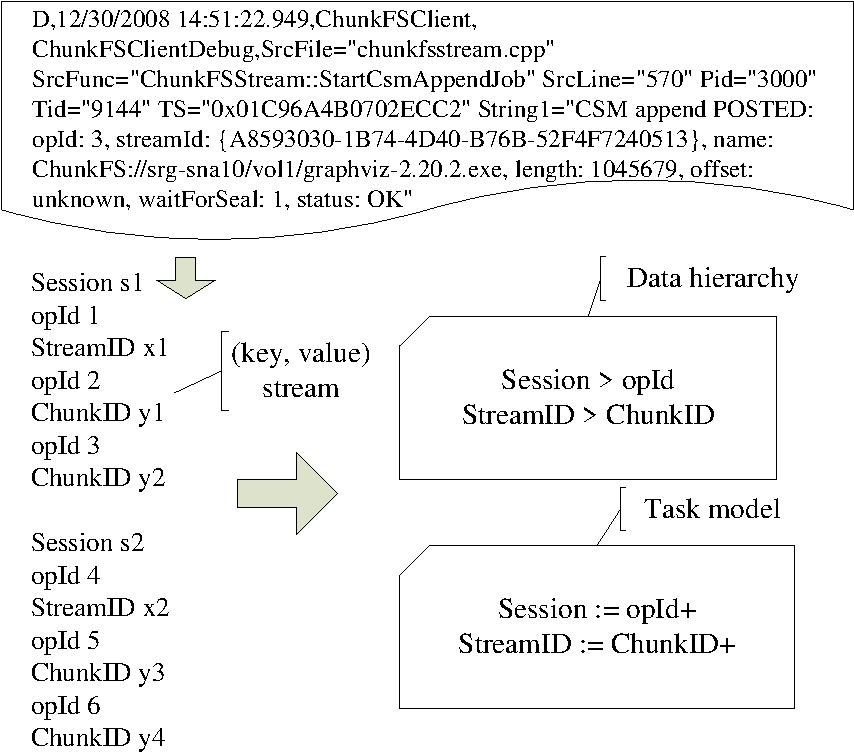
\includegraphics[height=2.4in]{design}
\caption{Design Overview}
\label{fig:design}
\end{figure}

Our design is summarized in Figure~\ref{fig:design}. We
first extract data from system logs as streams of (key,
value) tuples. Then we try to mine hierarchical relations
among keys. The mined relations can be directly translated
to task models. Applying the task models on logs, we
generate a set of task instances represented as an array of
log items.


\subsection{Extract key-value pairs}

System logs contains a lot of information on system
activities. The log items mainly describes who (threads,
event handlers) are performing some operations (as function
name or in human language) on a set of data, with extra
information such as operation result (return code).

Our tool can infer the hierarchical relations among the data
on which system operates and generate task models using
inferred data hierarchy.

To do the inference, we have to first extract data part
from log. It will be represented as (key, value) tuples,
with key as data identifer and value as current content.

Different system have different log format. We describe how
to extract data from \cosmos log in (key, value) form. The
principle described here can be adopted to analyze other
kinds of log.

\begin{figure}
\begin{verbatim}
d,12/30/2008 14:51:22.949,ChunkFSClient,
ChunkFSClientDebug,SrcFile="ChunkFSstream.cpp"
SrcFunc="ChunkFSStream::StartCsmAppendJob"
SrcLine="570" Pid="3000" Tid="9144"
TS="0x01C96A4B0702ECC2" String1="CSM append
POSTED: opId: 3, streamId:
{A8593030-1B74-4D40-B76B-52F4F7240513}, name:
chunkfs://srg-sna10/vol1/graphviz-2.20.2.exe,
length: 1045679, offset: unknown,
waitForSeal: 1, status: OK"
\end{verbatim}
\caption{A sample log item}
\label{fig:logitem}
\end{figure}

The Figure~\ref{fig:logitem} shows a typical log item picked
from \cosmos.  The \cosmos log can be divided into two parts.
The first half has fixed format, which records log level,
time, log category and a short title. Followed by the
location of the log in source file, and runtime parameters.
The second half is contained in \texttt{String1} field. It
is written by developer and not well structured. It is
usually interleaved with descriptive texts and programs
states in (key, value) pairs.

It is not straightforward to extract the (key, value) pairs.
The developer can record (key, value) in several formats. In
general, it is written as \texttt{key SEP1 value SEP2}. SEP1
and SEP2 have multiple choices. It is not easy to determine
which word is a key, otherwise we can do the job easily. A
key may look similar to an irrelevant words, such as
\texttt{POSTED:} and \texttt{opId:}.

We use a novel method to extract the (key, value) pairs. It
is based on the observation that the value part has limited
formats, such as an integer, a hexadecimal or a GUID, and it
is easy to be match by regular expression. Once the value
part is located, we can track back in the text to find its
corresponding key.

Currently, we choose to extract (key, value) pairs whose
value parts are numbers but not text. Our considerations
are: a) values as text are more descriptive and have
little use in inferring data hierarchy in later steps. b)
SEP1 and SEP2 may be both blanks. In such cases,
text words, keys and values are messed up and they cannot be
distinguished using simple rules.

In verifying the extracted (key, value) pairs, we note that
there are cases where 1) a key may have multiple alias names,
2) different keys may share the same name. We use a mapping
schema to solve the both problems. After a log item is
parsed, we apply the mapping specified in schema file and
translate some keys to a new name.

The schema specify mappings as (SrcFile, SrcFunc, key) $\to$
(new key). In this way, key aliases can be solved by
writing (*, *, alias) $\to$ (key). And key confliction can
be solved by writing (SrcFileX, SrcFuncY, conflict key) $\to$
(new key). In our experiences, just specifying SrcFuncY is
enough.

Our method for extracting data from log have limitations. It
recognizes key as the previous word of a value. It is based
on observations from logs and the observation reflects
developers logging practice. Several other choices are
available. We can improve the logging facility to support
structured data recording, or we can leverage NLP techniques
to extract data more precisely.

\subsection{Mining hierarchical relation of keys}

Some of the keys extracted from log have hierarchy
relations. For example, to complete a \texttt{Session}, it
is splitted into subtasks which are designated by different
\texttt{opId}. There are similar relations with
\texttt{StreadID} and \texttt{ChunkID}. We can use the data
hierarchy to deduce task hierarchy. Two keys have
hierarchical relations are denoted by $>$ relation, for
example, \texttt{Session} $>$ \texttt{opId}.

After the previous step, we get a stream of (key, value)
pairs in their order of appearance in log file. Activities
from multiple threads may be logged into the same log file.
We split (key, value) streams by thread and mine different
sub-streams separately. The mined results are combined
together.

We use two heuristics to mine data hierarchy among keys.
They are the necessary conditions for two keys to have
hierarchical relation.
\begin{itemize}
\item If keyS $>$ keyP, then keyS comes before keyP.
\item If keyS $>$ keyP, then there're strict 1-to-many
mapping between keyS and keyP value set.
\end{itemize}
The intuition is, if keyS $>$ keyP, one will see keyS first,
and a series of keyP with different values, and then keyS,
with another value, and then a series of keyP.

The mining algorithm takes (key, value) stream as input and
outputs (keyS, keyP, R) tuples, indicating keyS $>$ keyP
with rank R.

\begin{figure}
\centering
\begin{verbatim}
Session s1
opId 1
StreamID x1
opId 2
ChunkID y1
opId 3
ChunkID y2

Session s2
opId 4
StreamID x2
opId 5
ChunkID y3
opId 6
ChunkID y4
\end{verbatim}
\caption{A sample (key, value) stream}
\label{fig:kvstream}
\end{figure}

Figure~\ref{fig:kvstream} emulate the (key, value) stream we
see in \cosmos client log. When the client receives a
command, it starts a new session, opens the specified stream
in next operation step, and process chunks of the stream in
the following operation steps.

The rank algorithm works as follows. It scans through the
(key, value) stream and maintains an array of keys. Once a
key is spotted for the first time, it is appended to the key
array. A key is a possible parent for all the keys after it
in the array (heuristic 1). In the scan process, the algorithm also
accumulate an array of (valueS, valueP) for each (keyS, keyP)
pairs. A new (keyP, valueP) will generate multiple (valueS,
valueP) pairs for each keyS before keyP in the key array.

Now for each (keyS, keyP) pair, we have a corresponding
(valueS, valueP) array. To apply heuristic 2, we have to
justify whether valueS and valueP have strict 1-many
mappings. If yes, we use size of (valueS, valueP) array
as the rank of (keyS, keyP), if not, we just ignore the
(keyS, keyP) pair.

\notes{pseudo code of mining algorithm}

For sample (key, value) stream in Figure~\ref{fig:kvstream},
we sucessfully mined out StreamID $>$ ChunkID with rank 4
and Session $>$ opId with rank 6. Session has no relation
with StreamID, because multiple Session may operate on the
same StreamID. The similar argument apply for (Session,
ChunkID), (opId, StreamID) and (opId, ChunkID).

For (key, value) streams generated form real world log, the
mined result may contain a lot false positives. Because we
just put every key we extract from log into mining
algorithm.

By looking at false positive results, we recognize that keys
can be roughly divided into two categories, \notes{xxx}

\subsection{Construct hierarchical task models}

After the previous step, we mined out a set of data
hierarchy relations. The relations can be translated
directly to hierarchies of tasks which process the data.
If we have keyS $>$ keyP, and use Task(keyS) to denote task
that process keyS, then we have Task(keyS) $:=$
Task(keyP)$+$, in short keyS $:=$ keyP+. We use the later
definition as task model.

We apply the mined data hierarchy on the log to split system
runtime into hierarchical task instances. Each task instance
is represented by a sequence of log items describing system
activities within a certain time interval of the same
thread. We first split log items into first level task
instances by highest level key. An instance begins at the
new value of the key is spotted and last until another value
is met. We apply the process recursively within each first
level instances to obtain lower level task instances.

\begin{figure}
\centering
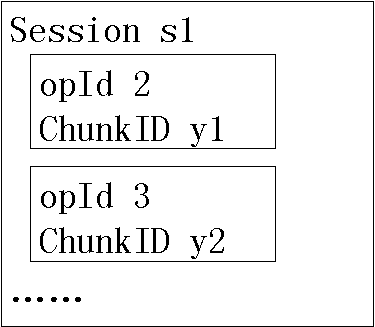
\includegraphics[height=1.5in]{runtime}
\caption{Hierarchical task instances.}
\label{fig:runtime}
\end{figure}

For \cosmos client, we find it convenient to using Session
$:=$ opId$+$ as task model. This is consistent with
developer's mind on organizing client activities. After
applying the model on (key, value) streams in
Figure~\ref{fig:kvstream}, we organize the activities as in
Figure~\ref{fig:runtime}.

The choice of which data hierarchy to apply is left to user.
The choice depends on user's concentration. The user are not
limited to mined result. Other hierarchy relations can be
specified. For example, one can combine Session, opId,
StreamID, ChunkID together, and write the relation as
Session $:=$ opId$+$, opId $:=$ StreamID$|$ChunkID.

After we obtain task instances, we use value-based joins to
draw dependency lines among tasks.

